\documentclass[numbers,handout]{ximera}
%% handout
%% nohints
%% newpage

\input{preamble.tex}

\let\masterdocument\document
\let\endmasterdocument\enddocument



\begin{masterdocument}
\begin{titlepage}
    \vspace*{1in}
    \begin{center}
      {\Huge \bfseries History of mathematics}\\[0.5cm]
      {\Large Bart Snapp}\\[0.4cm]
      This document was typeset on \today.
    \end{center}
    %\vspace*{\fill}
  \end{titlepage}

\tableofcontents

\renewcommand{\documentclass}{\setbox0\vbox}
\renewcommand{\preambleinput}{\setbox0\vbox}
\renewenvironment{document}{}{}

\documentclass{ximera}

\input{../preamble.tex}

\prerequisites{algebra}
\outcomes{conceptOfNumber}

\title{What is a number?}
\begin{document}
\begin{abstract}
In this activity we think about what it means to be a number.
\end{abstract}
\maketitle

\begin{question}
What is a number? List out some qualities that you think a number has.
\end{question}

\begin{question}
How do you know when something is not a number?
\end{question}

\begin{question}
What are different ways we could represent numbers?
\end{question}

\begin{question}
What if we used the following system:
\[
1 = a, \quad 2 = aa, \quad 3 = aaa, \quad\text{and so on.}
\]
What does the word \textit{concatenation} mean? How does it apply to
this system?  How would we add? How would we multiply? How could we
represent negative numbers?
\end{question}


\begin{question}
Once Oscar wondered what the number $\pi$ was. So he typed it into his
calculator and found:
\[
\pi = 3.1415926\dots
\]
Oscar then exclaimed, ``Ah now I know what number $\pi$ is.'' Can you
explain Oscar's thoughts on numbers?
\end{question}


\begin{exercise}
What are the 7 basic ancient Egyptian numerical symbols and what do
they mean?
\end{exercise}


\begin{question}
Is this ancient Egyptian system a place-value system or a
concatenation system? Explain your reasoning.
\end{question}


\begin{question}
Suppose you wanted to write out all the numbers from 1 to 1000000. How
many distinct symbols would you need if using the ancient Egyptian
system? How many distinct symbols would you need if using our system?
How many symbols would the longest string require? 
\end{question}

\begin{question}
Is there a simple rule for multiplying by 10 in the ancient Egyptian system?
\end{question}
\end{document}

\documentclass{ximera}

\input{../preamble}


\prerequisites{algebra}
\outcomes{egyptianFractions,placeValue}

\title{Measuring with fractions}
\begin{document}
\begin{abstract}
In this activity we will explore Egyptian fractions.
\end{abstract}
\maketitle

Here is a basic question for you: 

\begin{question}
What is the smallest number of weights needed to produce every
integer-valued mass from $0$ grams to say $n$ grams? Explain your
reasoning.
\end{question}

Now suppose that you want to measure all fractions of a given unit
with unit fractions. 

\begin{exercise}
Express 
\[
\frac{2}{5}, \qquad \frac{3}{5}, \qquad \frac{4}{5} 
\]
as the sum of unit fractions. 
\end{exercise}

Why would somebody work with such beasts? I'm not sure, but I have two
guesses. 

First guess: Egyptians weren't using fractions for fun, they wanted to do
real measurements. One could imagine a market where to measure weights
one has a balance. If you had a fixed set of weights that allowed you
to measure many different types of fractional weights, the
decomposition of a fraction into unit sums would be of interest.

Second guess: It has to do with distributing in a real world setting.

\begin{question}
Suppose you have 7 loafs of bread that you wish to share among 8
people. How much of a loaf of bread do you need to give each person?
How \textbf{exactly} do you distribute the bread?
\end{question}


\begin{exploration}
Express 
\[
\frac{2}{7}, \qquad \frac{3}{7}, \qquad \frac{4}{7}, \qquad\frac{5}{7}, \qquad\frac{6}{7} 
\]
as the sum of unit fractions. Can you give a general method?
\end{exploration}
\end{document}

\input{./theMethodOfFalsePosition/theMethodOfFalsePosition.tex}
\documentclass[handout,newpage]{ximera}

%\prerequisites{algebra}
%\outcomes{placeValue,squareRoots}
\input{../preamble.tex}


\title{Babylonian numbers} 


\begin{document}
\begin{abstract}In this activity we explore the number system of the ancient
  Babylonians.
\end{abstract} 
\maketitle


The ancient Babylonians used cuneiform characters to write their
numbers.

\begin{exercise}
What are the 2 basic ancient Babylonian numerical symbols and what do
they mean?
\end{exercise}


\begin{exercise}
Express the numbers 
\[
1, \qquad 7,\qquad 13,\qquad 53,\qquad 101 
\]
as the ancient Babylonians would. 
\end{exercise}


\begin{question}
Express 0 as the ancient Babylonians would. 
\end{question}


\begin{question}
Count from 58 to 62 using the ancient Babylonian symbols. 
\end{question}



\begin{exploration}
Express the numbers 
\[
11,\qquad 660,\qquad 39600 
\]
as the ancient Babylonians would. 
\end{exploration}


\begin{exploration}
Discuss the limitations of the Babylonian system. Then debate whether
these so-called limitations were actually limitations at all.
\end{exploration}

\begin{exploration}
Is the Babylonian system more of a place-value system or a
concatenation system?
\end{exploration}



\begin{question}%% note difficult problem from math through ages
Express the numbers 
\[
\frac{5}{6}, \qquad \frac{1}{20},\qquad \frac{1}{100}
\]
in sexagesimal notation.
\end{question}



\begin{question}
Here is a computation of how ancient Babylonians approximated square
roots---without any explanation!
\begin{enumerate}
\item $\sqrt{26}> 5$
\item $5 \cdot \frac{26}{5} = 26$
\item $\frac{26}{5}> \sqrt{26}$
\item $\sqrt{26}\approx \frac{5+\frac{26}{5}}{2}$
\end{enumerate}
Explain the algorithm used and give another example to show you know how it
is done.
\end{question}

\begin{exploration}
When is this approximation a good approximation?
\end{exploration}

\end{document}

\input{./rationalNumbersAndSimilarity/rationalNumbersAndSimilarity.tex}
\input{./pythagoreanMeans/pythagoreanMeans.tex}
\input{./computingQuadratures/computingQuadratures.tex}
\documentclass{ximera}

\prerequisites{geometry}
\outcomes{quadratures}

\preambleinput{../preamble.tex}

\title{Squaring the circle with lunes}
\begin{document}
\begin{abstract}
In this activity we investigate a proposed method of squaring the circle.
\end{abstract}
\maketitle

It is impossible to square the circle with compass and straightedge
alone. However, it is still interesting to think about what one's
strategy might be to achieve this impossible goal. We will work with a
circle of diameter $D$.
\begin{image}
\begin{tikzpicture}[geometryDiagrams]
\draw (0,0) circle (1cm);
\draw[thin] (-1,0)--(1,0);
\node at (0,-.2) {$D$};
\end{tikzpicture}
\end{image}


\begin{question}
Consider a circle of \textbf{radius} $D$. What is the relationship
between the area of the original circle and this new circle?
\end{question}


\begin{question}
Consider a circle of \textbf{radius} $D$. We claim that we can
inscribe a regular hexagon of side length $D$ in this circle.
\begin{image}
\begin{tikzpicture}[geometryDiagrams]
\draw[thin] (0,0) circle (2cm);
\draw (2,0)--({2*cos(60)},{2*sin(60)});
\draw ({2*cos(60)},{2*sin(60)})--({2*cos(120)},{2*sin(120)});
\draw ({2*cos(120)},{2*sin(120)})--({2*cos(180)},{2*sin(180)});
\draw ({2*cos(180)},{2*sin(180)})--({2*cos(240)},{2*sin(240)});
\draw ({2*cos(240)},{2*sin(240)})--({2*cos(300)},{2*sin(300)});
\draw ({2*cos(300)},{2*sin(300)})--(2,0);
\draw[decoration={brace,raise=.2cm},decorate,thin] ({2*cos(120)},{2*sin(120)})--({2*cos(180)},{2*sin(180)});

\node at (-1,.6) {$D$};
\end{tikzpicture}
\end{image}
Explain how you know this is true.
\end{question}


\begin{question}
Still considering a circle of \textbf{radius} $D$, add some lunes.
\begin{image}
\begin{tikzpicture}[geometryDiagrams]
\draw (0,0) circle (2cm);
\draw[thin] (2,0)--({2*cos(60)},{2*sin(60)});
\draw[thin] ({2*cos(60)},{2*sin(60)})--({2*cos(120)},{2*sin(120)});
\draw[thin] ({2*cos(120)},{2*sin(120)})--({2*cos(180)},{2*sin(180)});
\draw[thin] ({2*cos(180)},{2*sin(180)})--({2*cos(240)},{2*sin(240)});
\draw[thin] ({2*cos(240)},{2*sin(240)})--({2*cos(300)},{2*sin(300)});
\draw[thin] ({2*cos(300)},{2*sin(300)})--(2,0);

\draw (2,0) arc (-60:120:1cm);
\draw ({2*cos(60)},{2*sin(60)}) arc (0:180:1cm);
\draw ({2*cos(120)},{2*sin(120)}) arc (60:240:1cm);
\draw ({2*cos(180)},{2*sin(180)}) arc (120:300:1cm);
\draw ({2*cos(240)},{2*sin(240)}) arc (180:360:1cm);
\draw ({2*cos(300)},{2*sin(300)}) arc (-120:60:1cm);
\end{tikzpicture}
\end{image}
Now write two expressions for the area of the entire figure, one built
from the area of a regular hexagon and the area of the original
circle, and the other built from the area of the larger circle and the
area of the lunes.
\end{question}

\begin{question}
Explain how this gives a method for finding the quadrature of a
circle, assuming you know how to find the quadrature of lunes.
\end{question}

\end{document}

\documentclass{ximera}

\input{../preamble.tex}

\title{Euclid's Elements}

\begin{document}
\begin{abstract}
Here we see the beginning and some selections from
Euclid's \textit{Elements}.
\end{abstract}
\maketitle


Here is an excerpt from Euclid's \textit{Elements}. We have adapted
this from the edition by Richard
Fitzpatrick\link{http://farside.ph.utexas.edu/books/Euclid/Euclid.html}.




{\setlength{\parindent}{0pt}
\subsection*{Definitions}

1.~A point is that of which there is no part.

2.~And a line is a length without breadth.

3.~And the extremities of a line are points.

4.~A straight-line is (any) one which lies  evenly with points on itself.

5.~And a surface is that which has length and breadth only.

6.~And the extremities of a surface are lines.

7.~A plane surface is (any) one which lies evenly with the straight-lines on itself.

8.~And a plane angle is the inclination of the lines to one another, when two lines in a plane 
meet one another, and are not lying in a straight-line.

9.~And when the lines containing the angle are straight then the angle is called rectilinear.

10.~And when a straight-line stood upon (another) straight-line makes adjacent angles (which are) equal to one another, each of the equal angles is a
right-angle, and the former straight-line  is called a perpendicular to that upon which it stands.

11.~An obtuse angle is one greater than a right-angle.

12.~And an acute angle (is) one less than a right-angle.

13.~A boundary is that which is the extremity of something.

14.~A figure is that which is contained by some boundary or boundaries.

15.~A circle is a plane figure  contained by a single line [which is called a circumference], (such that) all of the straight-lines  radiating towards
 [the circumference] from one
point amongst those lying inside the figure  are equal to one another.

16.~And the point is called the center of the circle.

17.~And a diameter of the circle is any straight-line, being drawn through the
center, and terminated in each direction by the circumference of the circle. (And) any such (straight-line) also cuts the circle in half.$^\dag$

18.~And a semi-circle is the figure contained by the diameter  and
the circumference  cuts off by it. And the center of the semi-circle is the same (point)
as (the center of) the circle.

19.~Rectilinear figures are those (figures) contained by straight-lines: trilateral
figures being those contained by three straight-lines,  quadrilateral   by four,
and multilateral by more than four.

20.~And of the trilateral figures: an equilateral triangle is that having
three equal sides, an isosceles (triangle) that having only two equal sides,
and a scalene (triangle) that having three unequal sides.

21.~And further of the trilateral figures: a right-angled triangle is that having
a right-angle, an obtuse-angled  (triangle) that having an obtuse
angle, and an acute-angled (triangle) that having three acute angles.

22.~And of the quadrilateral figures: a square is that which is right-angled
and equilateral, a rectangle that which is right-angled but not equilateral,
a rhombus that which is equilateral but not right-angled, and a rhomboid that
having opposite sides and angles equal to one another which is neither
right-angled nor equilateral. And let quadrilateral figures besides these be called
trapezia.

23.~Parallel lines are straight-lines which, being in the same plane, and
being produced to infinity in each direction, meet with one another in
neither (of these directions).

\subsection*{Postulates}

1.~Let it have been postulated to draw a straight-line from any point to any point.

2.~And to produce a finite straight-line continuously in a straight-line.

3.~And to draw a circle with any center and radius.

4.~And that all right-angles are equal to one another.

5.~And that if a straight-line falling across two (other) straight-lines makes 
internal angles on the same side (of itself whose sum is) less than two right-angles, then the two (other) straight-lines, being produced to infinity, meet on that side (of the original straight-line) that the (sum of the internal angles) is less
than two right-angles (and do not meet on the other side).



\subsection*{Common Notions}

1.~Things equal to the same thing are also equal to one another.

2.~And  if equal things are added to equal things then the wholes are equal.

3.~And if equal things are subtracted from equal things then the remainders are
equal.

4.~And things coinciding with one another are equal to one another.

5.~And the whole [is] greater than the part.

}


\begin{proposition}[I.15]
If two straight-lines cut one another then they make the vertically
opposite angles equal to one another.
\end{proposition}

\begin{question}
Can you prove Proposition I.15?
\end{question}

\begin{proposition}[I.16]
For any triangle, when one of the sides is produced, the external
angle is greater than each of the internal and opposite angles.
\begin{image}
\begin{tikzpicture}[geometryDiagrams]
\coordinate (A) at (0,2);
\coordinate (B) at (2,5);
\coordinate (C) at (6.5,2);
\coordinate (F) at (9,2);
\draw (A)--(B)--(C)--cycle;
\draw (C)--(F);
\tkzLabelPoints[above](B)
\tkzLabelPoints[below](A,C)
\tkzMarkAngle[size=0.5cm,thin](F,C,B)
\tkzLabelAngle[pos = 0.25](F,C,B){$\epsilon$}

\tkzMarkAngle[size=0.6cm,thin](A,B,C)
\tkzLabelAngle[pos = 0.35](A,B,C){$\beta$}

\tkzMarkAngle[size=0.6cm,thin](C,A,B)
\tkzLabelAngle[pos = 0.35](C,A,B){$\alpha$}

%\draw[step=.5cm] (0,0) grid (10,5);
\end{tikzpicture}
\end{image}
\end{proposition}

\begin{question}
Can you prove Proposition I.16?
\end{question}

\begin{proposition}[I.27]
If a straight-line falling across two straight-lines makes the
alternate angles equal to one another then the (two) straight-lines
will be parallel to one another.
\end{proposition}


\begin{question}
Can you prove Proposition I.27?
\end{question}


\begin{proposition}[I.29]
A straight-line falling across parallel straight-lines makes the
alternate angles equal to one another, the external (angle) equal to
the internal and opposite (angle), and the (sum of the) internal
(angles) on the same side equal to two right-angles.
\end{proposition}


\begin{question}
Can you prove Proposition I.29?
\end{question}


\begin{proposition}[I.32]
In any triangle, (if) one of the sides (is) produced (then) the
external angle is equal to the (sum of the) two internal and opposite
(angles), and the (sum of the) three internal angles of the triangle
is equal to two right-angles.
\end{proposition}


\begin{question}
Can you prove Proposition I.32?
\end{question}
\end{document}

\documentclass{ximera}

\input{../preamble.tex}

\title{Triangles on a Cone}	
\begin{document}
\begin{abstract}
In this activity we investigate the sum of the interior angles of a triangle.
\end{abstract}
\maketitle


\subsection*{Euclidean geometry}

We are going to investigate why the interior angles of a triangle sum
to $180^\circ$. We won't be alone on this journey; we'll have help.
Meet Louie Llama:\index{Louie Llama}
\begin{image}
\includegraphics[height=1in]{llama.pdf}
\end{image}

Louie Llama is rather radical for a llama and doesn't mind being
rotated.

\begin{question} 
Draw a picture of Louie Llama rotated $90^\circ$ counterclockwise.
\end{question}

\begin{question} 
Draw a picture of Louie Llama rotated $180^\circ$ counterclockwise.
\end{question}

\begin{question} 
Draw a picture of Louie Llama rotated $360^\circ$ counterclockwise.
\end{question}

\begin{question} Sometimes Louie Llama likes to walk around lines he finds:
\begin{image}
\includegraphics{llamaLines.pdf}
\end{image}
Through what angle did Louie Llama just rotate?
\end{question}


Now we're going to watch Louie Llama go for a walk. Draw yourself any
triangle.  Actually, draw a crazy scalene triangle---those are the kind that Louie
Llama likes best. Louie Llama is going to proudly parade around this
triangle. When Louie Llama walks around corners he rotates. Check
it out:
\begin{image}
\includegraphics{llamaCorner.pdf}
\end{image}
Take your triangle and denote the measure of its angles as $a$, $b$,
and $c$. Start Louie Llama out along a side adjacent to the angle of
measure $a$. He should be on the outside of the triangle, his feet
should be pointing toward the triangle, and his face should be
pointing toward the angle of measure $b$.
\begin{question} 
Sketch Louie Llama walking to the angle of measure $b$. Walk him
around the angle. As he goes around the angle his feet should always
be pointing toward the triangle. Through what angle did Louie Llama
just rotate?
\end{question}

\begin{question}
Sketch Louie Llama walking to the angle of measure $c$. Walk him
around the angle. Through what angle did Louie Llama just rotate?
\end{question}

\begin{question}
Finally, sketch Louie Llama walking back to the angle of measure
$a$. Walk him around the angle. He should be back at his starting
point. Through what angle did Louie Llama just rotate?
\end{question}

\begin{question} 
All in all, how many degrees did Louie Llama rotate in his walk?
\end{question}

\begin{question} 
Write an equation where the right-hand side is Louie Llama's total
rotation and the left-hand side is the sum of each rotation around the
angle. Can you solve for $a+b+c$?
\end{question}



\subsection*{A noneuclidean geometry}


Put a dot at the center of a blank sheet of paper and call it $O$.
Use a protractor to draw an angle of $50^\circ$ with vertex at the
point $O$ and sides extending all the way out to the edge of the
paper.  Cut the paper along one side of the angle and one side only.
Make a cone by moving the cut edge to the other side of the angle you
drew.  This cone (extended infinitely) is your universe.


\begin{question}
Make a triangle in your universe that surrounds $O$. To do this,
unfold your universe and lay it out flat on the desk and make the
sides with your ruler.  When a side gets to the cut side of your
angle, put the other side of the angle on top and keep going.
\end{question}

\begin{question}
You measure angles on your universe by laying the paper out flat and
measuring the angles on the paper. Measure the angles in your
triangle, what do they sum to?
\end{question}


\begin{question}
Repeat the questionlems above, but this time cut an angle of $40^\circ$ to
make your cone. What do you notice?
\end{question}

Let's see if we can explain this. Do you know who is eager to help
you? That's right: Louie Llama.
\begin{image}
\includegraphics[height=1in]{llama.pdf}
\end{image}

\begin{question}
Take your triangle and denote the measure of its angles as $a$, $b$,
and $c$. We would like to parade Louie around the triangle. There is
only one catch: What happens to Louie when he passes over the ``cut?''
Draw some pictures and see if you can figure it out.
\end{question}

Start Louie Llama out along a side adjacent to the angle of measure
$a$. He should be on the outside of the triangle, his feet should be
pointing toward the triangle, and his face should be pointing toward
the angle of measure $b$. Continue this process and walk him all
around the triangle. When he gets to the ``cut'' put the paper
together, and let him continue his walk.

\begin{question} 
Through what angle does Louie rotate when he strolls around a vertex?
\end{question}

\begin{question}
How many degrees did the ``cut'' rotate Louie? 
\end{question}

\begin{question} 
All in all, how many degrees did Louie Llama rotate in his walk?
\end{question}


\begin{question}
If a cone is made on a sheet of paper with a cut of $\theta$ degrees,
and a triangle is made surrounding the point of the cone, what is the
sum of the degrees of this triangle?
\end{question}




\begin{question}
Explain why not all of Euclid's postulates could hold in this
universe. Exactly which postulates don't hold?
\end{question}
\end{document}

\documentclass{ximera}

\input{../preamble.tex}

\title{The Pythagorean Theorem}
\begin{document}
\begin{abstract}
In this activity we will see some proofs of the most famous theorem of
  all.
\end{abstract}
\maketitle



\begin{question}
Remind us, what is the most famous theorem of all and what exactly
does it assert?
\end{question}




\subsection*{Proofs by picture}



\begin{question}
Check out:
\begin{image}
\includegraphics{pbppyth1.pdf}
\end{image}
How does the picture above ``prove'' the Pythagorean Theorem?
\end{question}


\begin{question}
Explain how the following picture ``proves'' the Pythagorean Theorem.
\begin{image}
\includegraphics{pbpdilation.pdf}
\end{image}
\end{question}


\begin{question}
Check out this tessellation involving $2$ squares:
\begin{image}
\includegraphics{pbppyth2.pdf}
\end{image}
How does the picture above ``prove'' the Pythagorean Theorem?
\end{question}





\subsection*{Euclid's proof}


\begin{question} 
What would one need to prove about the following diagram to prove the
Pythagorean Theorem?
\begin{image}
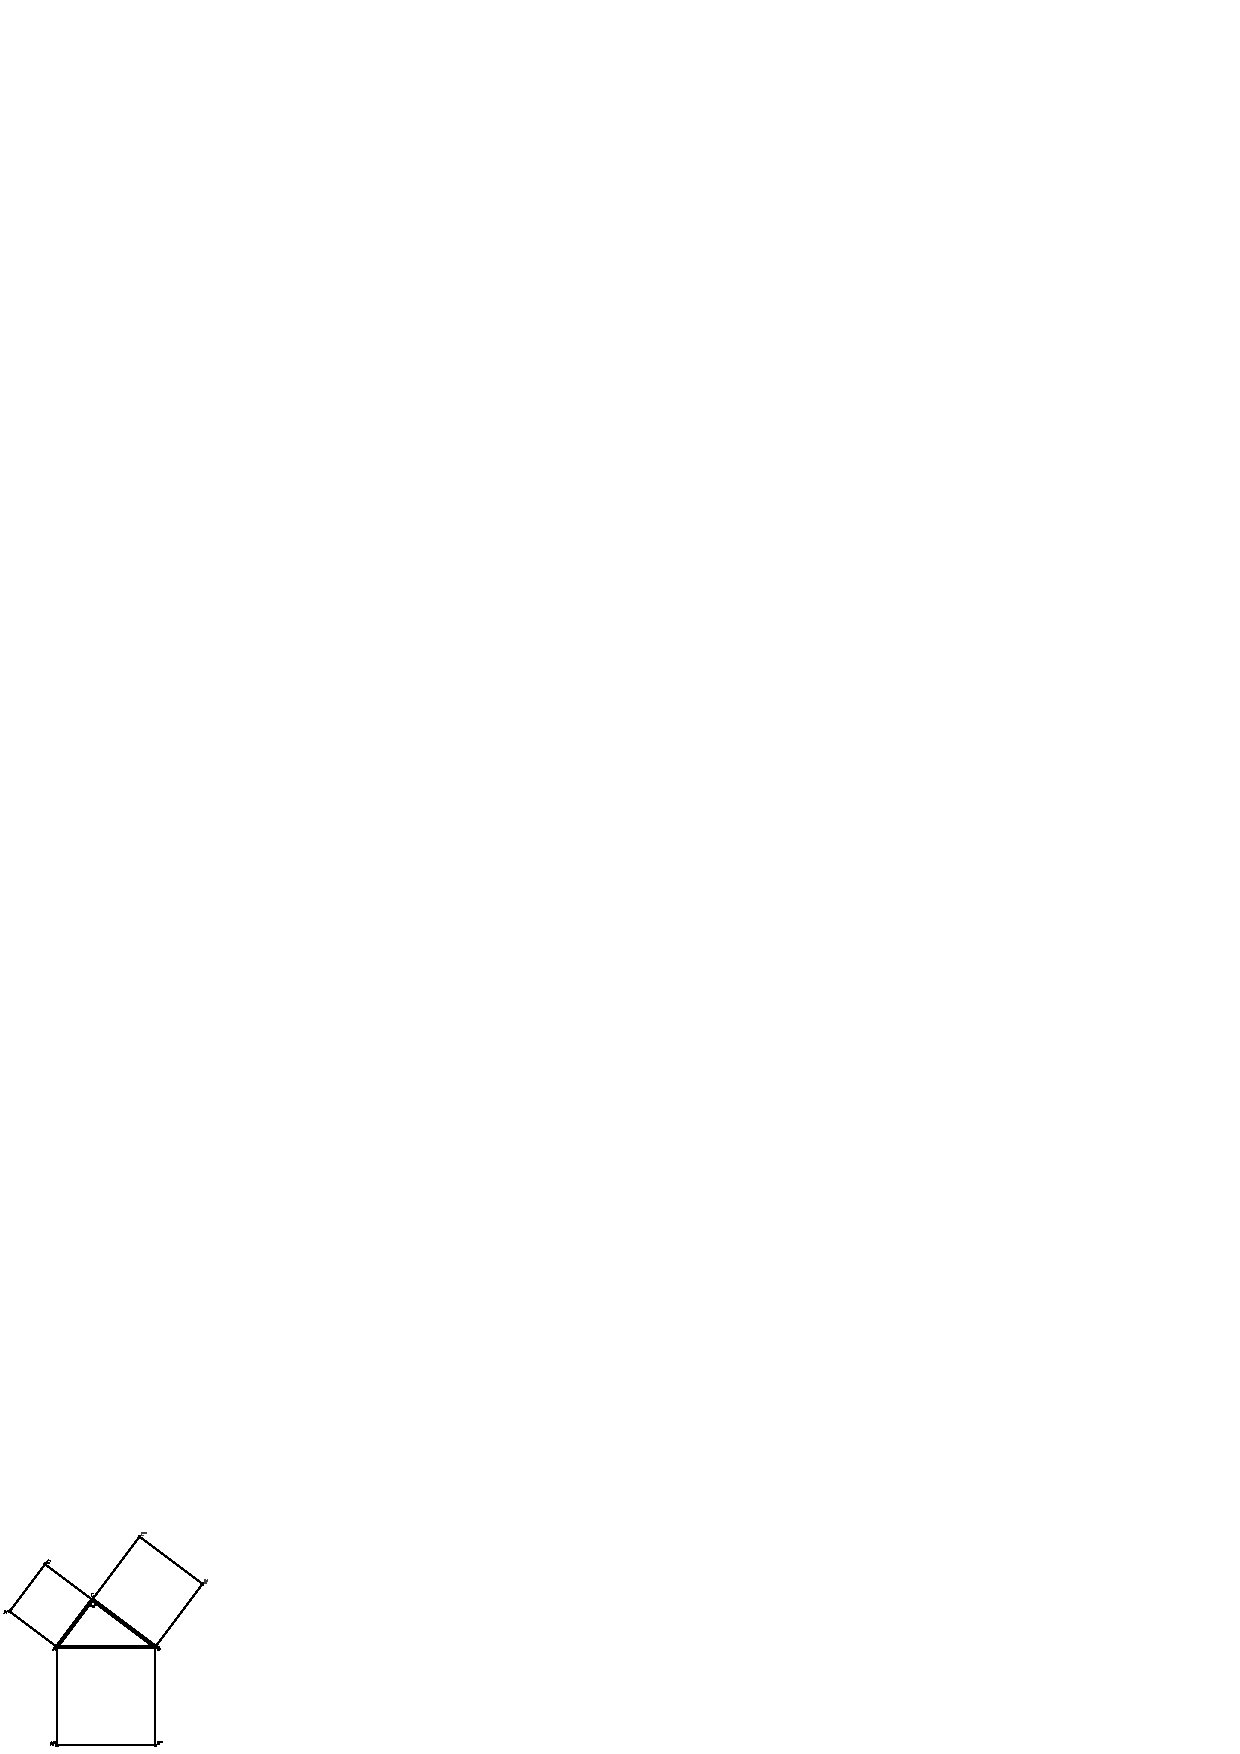
\includegraphics{PythEuclid.pdf}
\end{image}
\end{question}

Let's see if we can do this!


\begin{question}
Draw a line perpendicular to $\bar{AB}$ that passes though both $C$
and $\bar{A'' B''}$. Call the intersection between this line and
$\bar{AB}$, point $E$; call the intersection point between this line
and $\bar{A''B''}$, point $E'$. Explain why $\tri ACA''$ has half the
area of rectangle $AEE'A''$.
\end{question}

\begin{question}
Explain why $\tri ABA'$ has half the area of square $ACC'A'$.
\end{question}

\begin{question}
Explain why $\tri ACA''$ is congruent to $\tri ABA'$. 
\end{question}

\begin{question}
Explain why area of square $ACC'A'$ is equal to the area of rectangle
$AEE'A''$.
\end{question}


\begin{question}
Use similar ideas to complete a proof the Pythagorean Theorem.
\end{question}


\subsection*{The converse}

\begin{question} What is the converse to the Pythagorean Theorem? Is it true? How do you prove it?
\end{question}
\end{document}

\input{./theUniqueFactorizationTheorem/theUniqueFactorizationTheorem.tex}
\input{./heronsFormula/heronsFormula.tex}
\input{./solvingEquations/solvingEquations.tex}
\documentclass{ximera}


\input{../preamble}

\title{Complex Numbers From Different Angles}

\begin{document}
\begin{abstract}
In this activity we will investigate complex multiplication.
\end{abstract}
\maketitle




\begin{question} Consider the innocent little equation:
\[
x^3 -1 = 0
\]
How many solutions does it have? What are they? Plot them on the
complex plane below.
\[
\includegraphics{complexPlane.pdf}
\]
\end{question}

\begin{question}
Thinking about your work above, see if you can solve:
\[
x^4 -1 = 0
\]
Plot the solutions on the complex plane below.
\[
\includegraphics{complexPlane.pdf}
\]
\end{question}


\begin{question}
Suppose I told you that:
\begin{align*}
\sin(x) &= x - \frac{x^3}{3!} + \frac{x^5}{5!} - \frac{x^7}{7!} + \dots + \frac{(-1)^n x^{2n+1}}{(2n+1)!} + \cdots \\
\cos(x) &= 1 - \frac{x^2}{2!} + \frac{x^4}{4!} - \frac{x^6}{6!} + \dots + \frac{(-1)^n x^{2n}}{(2n)!} + \cdots \\
e^x &= 1 + x + \frac{x^2}{2!} + \frac{x^3}{3!} + \frac{x^4}{4!} + \dots + \frac{x^n}{n!} + \cdots 
\end{align*}
Explain why we say:
\[
e^{x\cdot i} = \cos(x) + i \sin(x)
\]
\end{question}

\begin{question}
 This is Euler's famous formula:
\[
e^{\pi \cdot i } + 1 = 0
\]
Use the questionlem above to explain why it is true.
\end{question}

\begin{question}
What does all this have to do with De Moivre's Theorem?
\end{question}

\begin{question}
How can you use this to take the $n$th root of a complex number?
\end{question}
\end{document}

\documentclass{ximera}

\input{../preamble.tex}

\title{De Moivre Saves the Day!}

\begin{document}
\begin{abstract}
Here we see how to take complex roots.
\end{abstract}
\maketitle


The rules for solving second and third degree equations led to a
``sticky wicket.''  Namely the rule for solving a quadratic equation
forced its user to take the square root of a number that was sometimes
negative.  Worse yet, the formula for solving a cubic equation forced
the user to take the cube root of a number that resulted from taking
square roots!  Despite misgivings, mathematicians were eventually
forced to expand the number system to one where square roots can be
found for any of its numbers.

You may recall that the Ferro-Tartaglia method gives 
\[
\sqrt[3]{\frac{-1+\sqrt{-31}}{2}} + \frac{2}{\sqrt[3]{\frac{1}{2}(-1+\sqrt{-31})}}
\]
as a solution to: $y = x^3-6x+1$. Moreover, as this plot of $y = x^3-6x+1$ shows
\[
\includegraphics[width=3in]{cubicPlot.pdf}
\]
this must be a real solution\dots But how? There is a square-root of a
negative number in the expression above! 

We're going to investiagate incredible connection between adding and
multiplying complex numbers and plane geometry.  It's called \textit{De
Moivre's rule}---it is here to save the day.  Please fasten your seat
belts and place your trays in the upright position.



You will need a scientific calculator and a straight-edge and compass.

\break

\begin{question}
Plot the point $(4,3)$ in the plane below---let each square be $1/2$
unit.  We will think of this point as the complex number $4 + 3i$.
\[
\includegraphics{complexPlane.pdf}
\]
\begin{enumerate}
\item Draw the ray from the origin through your chosen complex number.
\item Measure its distance to the origin (called the \textit{absolute value} of the complex number $4 + 3i$). 
\item Use inverse tangent to measure the angle between your complex number and the positive real axis. 
\end{enumerate}
\end{question}

\begin{question}
We're going to solve $(x+yi)^3 = 4+3i$ for $x$ and $y$ using geometry!
\begin{enumerate}
\item Compute the cube root of the absolute value you found before. 
\item Compute one-third of the angle you found before. 
\item Use sine and cosine to finish it off!
\item How can you check your work? Do it.
\end{enumerate}
\end{question}


\begin{question}
Now use De Moivre's method to take the cube roots found in:
\[
\sqrt[3]{\frac{-1+\sqrt{-31}}{2}} + \frac{2}{\sqrt[3]{\frac{1}{2}(-1+\sqrt{-31})}}
\]
\end{question}
\end{document}

\input{./theBinomialTheoremAndPi/theBinomialTheoremAndPi.tex}
\documentclass{ximera}

\input{../preamble.tex}

\title{Newton and Kepler}

\begin{document}
\begin{abstract}
In this activity we deduce Kepler's second law of planetary motion
from Newton's theory of gravitation.
\end{abstract}
\maketitle

In 1686, Isaac Newton published his book \textit{Philosophi\ae\
Naturalis Principia Mathematica}. This book contained Newton's theory
of gravitation:
\[
F = \frac{GMm}{R^2}
\] 
where $F$ is the magnitude of the force exerted between the masses, $M$ is the first (larger) mass, $m$ is the second (smaller) mass, $G$ is the gravitational constant, and $R$ is the distance between the centers of the masses. 

On the other hand in 1609, Kepler published his \textit{Second Law of
Planetary Motion}. This law states:
\begin{quote}
A line joining a planet and the Sun sweeps out equal areas during
equal intervals of time.
\end{quote}

One of the triumphs of Newton's theory of gravitation is that one can
actually deduce Kepler's laws (including the Second Law) from this
theory, Newton's \textit{Second Law of Motion}, and a bit of vector
calculus. Let's see how it's done. Note, we are giving a modern proof,
not the one Newton gave himself.

\begin{question}
Start with Newton's second law of motion, and explain the equation below:
\[
\vec{F} = m \vec{a} = m \frac{d^2\vec{R}}{dt^2} = \frac{-GMm}{|\vec{R}|^2}\cdot \frac{\vec{R}}{|\vec{R}|}
\]
\end{question}

\begin{question}
Explain why $\frac{d^2\vec{R}}{dt^2}$ is proportional to $\vec{R}$.
\end{question}

\begin{question}
Explain why 
\[
\vec{R} \times \frac{d^2\vec{R}}{dt^2} = \vec{0}.
\]
\end{question}

\begin{question}\label{Q:removeNaught}
Compute:
\[
\frac{d}{dt}\left(\vec{R}\times \frac{d\vec{R}}{dt}\right)
\]
and let:
\[
\vec{R}\times \frac{d\vec{R}}{dt}=\vec{C}
\]
What can you conclude about $\vec{C}$?
\end{question}


\begin{question}
Explain why $\vec{v}=\frac{d\vec{R}}{dt}$ and $\vec{R}$ lie in a plane
orthogonal to vector $\vec{C}$.
\end{question}

Let the plane containing $\vec{v}$ and $\vec{R}$ be the
$(x,y)$-plane. Let $\vec{k}$ be a unit vector in the direction of
$\vec{C}$. We will now switch to polar coordinates, where $t=0$ and
$\theta=0$ give direction of $\vec{R}$ when $|\vec{R}|$ is at a
minimum. Let $\vec{R}_0$ and $\vec{v}_0$ be the vector and velocity
corresponding to this minimum distance.

\begin{question}
Explain why 
\[
\vec{C} = \vec{R}_0\times \vec{v}_0.
\]
\end{question}


\begin{question}
Recalling that in polar coordinates
\begin{enumerate}
\item $\vec{R} = r\vec{u}_r$
\item $\vec{v} = \vec{u}_r \frac{dr}{dt} + \vec{u}_\theta \cdot r \frac{d\theta}{dt}$
\end{enumerate}
where (as usual for polar coordinates) $\vec{u}_r$ is a unit vector
pointing in the direction of the radius and $\vec{u}_\theta$ is a unit
vector perpendicular to the radius. Explain why
\[
\vec{C}=\vec{R}_0\times \vec{v}_0 = \vec{k} \left[r^2 \frac{d\theta}{dt}\right]_{t=0}= \vec{k} \cdot r_0v_0.
\]
\end{question}

\begin{question}
Now use Question~\ref{Q:removeNaught} to conclude
\[
\vec{k} \cdot r^2 \frac{d\theta}{dt}= \vec{k} \cdot r_0v_0
\]
\end{question}



\begin{question}
Recall in polar coordinates that area, $A$, is given by
\[
A = \frac{1}{2}\int_{\theta_0}^{\theta_1} r^2\d\theta. 
\]
Explain why if $\theta$ and $r$ are both functions of $t$, with
$\theta_0 = \theta(t_0)$ and $\theta_1 = \theta(t_1)$,
\[
A =  \frac{1}{2}\int_{\theta_0}^{\theta_1} r^2\d\theta = \frac{1}{2}\int_{t_0}^{t_1} r^2 \frac{d\theta}{dt} \d t 
\]
\end{question}


\begin{question}
Explain how this proves Kepler's Second Law:
\begin{quote}
A line joining a planet and the Sun sweeps out equal areas during equal intervals of time.
\end{quote}
Exactly which facts about the gravitational force did we use?
\end{question}
\end{document}

\input{./leibnizAndSeries/leibnizAndSeries.tex}
\input{./bernoulliEulerAndSeries/bernoulliEulerAndSeries.tex}
\input{./cantorCan/cantorCan.tex}

\end{masterdocument}
